\documentclass[12pt]{article}
\usepackage[utf8]{inputenc}
\usepackage{float}
\usepackage{amsmath}
\usepackage{amssymb}
\usepackage{tikz}

\usepackage[hmargin=3cm,vmargin=6.0cm]{geometry}
%\topmargin=0cm
\topmargin=-2cm
\addtolength{\textheight}{6.5cm}
\addtolength{\textwidth}{2.0cm}
%\setlength{\leftmargin}{-5cm}
\setlength{\oddsidemargin}{0.0cm}
\setlength{\evensidemargin}{0.0cm}

%misc libraries goes here
\usepackage{fitch}

\begin{document}

\section*{Student Information } 
%Write your full name and id number between the colon and newline
%Put one empty space character after colon and before newline
Full Name :  Alperen OVAK\\
Id Number :  2580801\\

% Write your answers below the section tags
\section*{Answer 1}

\paragraph{(a)}

\textbf{Base Case (\(n = 1\)):} 
When \(n = 1\), \(2^{3n} - 3^n = 2^3 - 3 = 8 - 3 = 5\), which is clearly divisible by 5.

\textbf{Inductive Step:}
Assume that for some positive integer \(k\), \(2^{3k} - 3^k\) is divisible by 5.

Now, let's show that it's true for \(k + 1\):

\[
\begin{aligned}
2^{3(k+1)} - 3^{k+1} &= 2^{3k + 3} - 3^{k+1} \\
&= 2^{3k} \cdot 2^3 - 3 \cdot 3^k.
\end{aligned}
\]

By our assumption, we know \(2^{3k} - 3^k\) is divisible by 5. Let \(2^{3k} - 3^k = 5m\) for some integer \(m\).

Now substitute this into our expression:

\[
\begin{aligned}
&= (5m+3^k) \cdot 2^3 - 3 \cdot 3^k \\
&= 40m +8\cdot 3^k - 3 \cdot 3^k.\\
&= 40m +5\cdot 3^k\\
&= 5(8m + 3^k).
\end{aligned}
\]

Since \(5(8m + 3^k)\) is divisible by 5, the entire expression is divisible by 5.

This completes the inductive step.

By mathematical induction, we've shown that \(2^{3n} - 3^n\) is divisible by 5 for all integers \(n \geq 1\).

\paragraph{(b)}

\textbf{Step 1 (Base Case):}
Show that the statement is true for \(n = 2\).

For \(n = 2\), we have:
\[4^2 - 7(2) - 1 = 16 - 14 - 1 = 1 > 0.\]
So, the base case holds.

\textbf{Step 2 (Inductive Step):}
Assume that the statement is true for some arbitrary positive integer \(k \geq 2\), i.e., assume that \(4^k - 7k - 1 > 0\).

Now, we need to show that the statement is also true for \(k + 1\). That is, we want to show:
\[4^{k+1} - 7(k+1) - 1 > 0.\]

Starting with the assumption \(4^k - 7k - 1 > 0\), let's manipulate this expression to get to \(4^{k+1} - 7(k+1) - 1\):

\[4^{k+1} - 7(k+1) - 1 = 4 \cdot 4^k - 7k - 7 - 1\]

Now, use the assumption \(4^k - 7k - 1 > 0\):

\[4^{k+1} - 7(k+1) - 1 = 4 \cdot (4^k) - 7k - 7 - 1 > 4 \cdot (7k + 1) - 7k - 7 - 1\]

Simplify further:

\[4 \cdot (7k + 1) - 7k - 7 - 1 = 28k + 4 - 7k - 8 = 21k - 4.\]

Now, since we assumed \(4^k - 7k - 1 > 0\) and, since \(k \geq 2\), we have \(21k - 4\) is greater than 0.
Therefore, we can say that \(4^{k+1} - 7(k+1) - 1 > 0 \).

Therefore, by mathematical induction, we have shown that \(4^n - 7n - 1 > 0\) for all integers \(n \geq 2\).

\section*{Answer 2}
\paragraph{(a)}

1. \textbf{Exactly 7 ones:}
   \[
   \binom{10}{7} = \frac{10!}{7!(10-7)!} = 120 \text{ combinations.}
   \]

2. \textbf{Exactly 8 ones:}
   \[
   \binom{10}{8} = \frac{10!}{8!(10-8)!} = 45 \text{ combinations.}
   \]

3. \textbf{Exactly 9 ones:}
   \[
   \binom{10}{9} = \frac{10!}{9!(10-9)!} = 10 \text{ combinations.}
   \]

4. \textbf{Exactly 10 ones:}
   \[
   \binom{10}{10} = \frac{10!}{10!(10-10)!} = 1 \text{ combination.}
   \]

Now, summing up these cases:
\[
120 + 45 + 10 + 1 = 176.
\]

So, there are 176 bit strings of length 10 with at least seven 1s in them.


\paragraph{(b)}

   Since the Discrete Mathematics textbooks and the Statistical Methods textbooks are both identical, which textbooks will be choosen does not matter.\\

   Also since we have a collection which we can assume it as a set, the order also does not matter.\\

   Therefore, we have jsut three posibilities with the condition that at least one Discrete Mathematics textbook and at least one Statistical Methods textbook is in the collection.\\

   Here is 3 posibilities:

1. \textbf{One Discrete Mathematics textbook and three Statistical Methods textbooks}
   
2. \textbf{Two Discrete Mathematics textbooks and two Statistical Methods textbooks}

3. \textbf{Three Discrete Mathematics textbooks and one Statistical Methods textbook}

\paragraph{(c)}

We know that there is \(3^5\) functions from from a set with 5 elements to a set with 3 elements. \\

To find onto functions, we should substract the number of non-onto functions from total number of functions.\\

Let's choose 2 elements in the domain, we have \(\binom{3}{2}\) posibilities. Then, we have \(2^5\) functions from a set with five elements to the remaining two elements in the each codomain. \\
\[
\binom{3}{2}2^5
\]

Let's choose 1 element in the domain, we have \(\binom{3}{1}\) posibilities. Then, we have \(1^5=1\) functions from a set with five elements to the remaining one element in the each codomain. 
Since first condition count this condition two times, we should add it up to the our result.\\
\[
\binom{3}{1}
\]

Therefore the result is:
\[
3^5 - \binom{3}{2}2^5 + \binom{3}{1} =150
\]

\section*{Answer 3}

\begin{figure}[h]
    \centering
    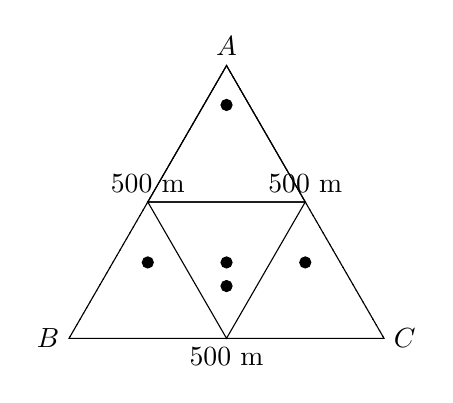
\begin{tikzpicture}
      % Vertices of the equilateral triangle
      \coordinate[label=above:$A$] (A) at (0,0);
      \coordinate[label=left:$B$] (B) at (-2, -3.464);
      \coordinate[label=right:$C$] (C) at (2, -3.464);

      \draw (A) -- (B) -- (C) -- cycle;
      
      \coordinate[label=above:$ $] (d) at (0,0);
      \coordinate[label=left:$ $] (e) at (-1, -1.732);
      \coordinate[label=right:$ $] (f) at (1, -1.732);

      % Draw the equilateral triangle
      \draw (d) -- (e) -- (f) -- cycle;

      \coordinate[label=above:$ $] (d) at (0,-3.464);
      \coordinate[label=left:$ $] (e) at (-1, -1.732);
      \coordinate[label=right:$ $] (f) at (1, -1.732);

      % Draw the equilateral triangle
      \draw (d) -- (e) -- (f) -- cycle;
  
      
      % Draw the distances for explanation
      \draw[dotted] (A) -- node[midway, above] {$500\text{ m}$} (B);
      \draw[dotted] (A) -- node[midway, above] {$500\text{ m}$} (C);
      \draw[dotted] (B) -- node[midway, below] {$500\text{ m}$} (C);
      
      \coordinate (E) at (0,-0.5);
      \draw[fill] (E) circle (2pt);
      \node[above right] at (E) {$ $};

      \coordinate (D) at (0,-2.5);
      \draw[fill] (D) circle (2pt);
      \node[above right] at (D) {$ $};

      \coordinate (F) at (-1,-2.5);
      \draw[fill] (F) circle (2pt);
      \node[above right] at (F) {$ $};

      \coordinate (G) at (1,-2.5);
      \draw[fill] (G) circle (2pt);
      \node[above right] at (G) {$ $};

      \coordinate (H) at (0,-2.8);
      \draw[fill] (H) circle (2pt);
      \node[above right] at (H) {$ $};
    \end{tikzpicture}
    \caption{Equilateral Triangle with Side Length 500 meters}
  \end{figure}
  
    This problem is a geometric version of the Pigeonhole Principle, In this case, each child represents a "pigeon," and the area within 250 meters of each child represents a "pigeonhole." The goal is to show that, no matter how the children are distributed within the equilateral triangle, at least two of them must be in the same "pigeonhole" (i.e., within 250 meters of each other). \\

    Let's, divide the triangle into four smaller equilateral triangles by connecting midpoints of its sides.(\( Figure 1 \))\\

    Then, the maximum distance between any two points within a small equilateral triangle is determined by the length of its side, which is 250 meters.\\

    So, no matter where the children are within the equilateral triangle, at least two of them will be within 250 meters of each other.\\

    This proves that, no matter how much the children wander within the triangle-shaped circus, there will always be two of them within 250 meters of each other.\\

\section*{Answer 4}
\textbf{a. Homogeneous Solution:}

The homogeneous part of the solution comes from ignoring the non-homogeneous term (in this case, \(5^{n-1}\)) and assuming a solution of the form \(a_n^{(h)} = c \cdot r^n\), where \(c\) is a constant and \(r\) is the characteristic root.

So, the homogeneous recurrence relation is \(a_n^{(h)} = 3a_{n-1}^{(h)}\).

Let \(a_n^{(h)} = c \cdot r^n\), then:

\[c \cdot r^n = 3c \cdot r^{n-1}\]

Divide both sides by \(c \cdot r^{n-1}\):

\[r = 3\]

So, the characteristic root \(r\) is 3.

The homogeneous solution is then:

\[a_n^{(h)} = c \cdot 3^n\]

\textbf{b. Particular Solution:}

The particular solution comes from the non-homogeneous term \(5^{n-1}\). Since this term is a constant multiplied by a power of 5, we can assume a particular solution of the form \(a_n^{(p)} = A \cdot 5^{n-1}\), where \(A\) is a constant.

Now, substitute this particular solution into the original recurrence relation:

\[A \cdot 5^{n-1} = 3(A \cdot 5^{n-2}) + 5^{n-1}\]

Solving for \(A\):

\[A = \frac{5}{2}\]

So, the particular solution is:

\[a_n^{(p)} = \frac{5}{2} \cdot 5^{n-1} = \frac{5^n}{2}\]

\textbf{c. Mathematical Induction:}

Let's find \(a_n\)

\[a_n = a_n^{(p)} + a_n^{(h)} \]

\[a_n = \frac{5^n}{2} + c \cdot 3^n \]

We know that \(a_1 = 4\):

\[a_1 = \frac{5^1}{2} + c \cdot 3^1 = 5/2 + 3c = 4\]

We find that \(c=0.5\).

Therefore, \[a_n = \frac{5^n}{2} + \frac{3^n}{2} \]

Now, we need to show by mathematical induction that the expression for \(a_n\) is a solution to the given recurrence relation.

\textbf{Base Case:}
For \(n = 1\), the initial condition is given as \(a_1 = 4\). Substituting \(n = 1\) into the expression for \(a_n\):

\[a_1 = \frac{5^1}{2} + \frac{3^1}{2} = 2.5 + 1.5 = 4\]

So, the base case holds. \\

\textbf{Inductive Step:}
Assume that \(a_k = \frac{5^k}{2} + 0.5 \cdot 3^k\) holds for some arbitrary \(k\).

Now, we want to show that \(a_{k+1} = \frac{5^{k+1}}{2} + 0.5 \cdot 3^{k+1}\) holds.

Substitute \(n = k+1\) into the expression for \(a_n\):

\[a_{k+1} = 3a_k + 5^k\]

\[= 3\left(\frac{5^k}{2} + 0.5 \cdot 3^k\right) + 5^k\]

\[= \frac{5^{k+1}}{2} + 1.5 \cdot 3^{k+1} + 5^k\]

\[= \frac{5^{k+1}}{2} + 0.5 \cdot 3^{k+1}\]

So, by mathematical induction, we have shown that the expression for \(a_n\) satisfies the given recurrence relation.


\end{document}